\section{Research Objectives and Milestones}
\label{sec:objectives}

We propose a multi-year progressive investigation of the CCSN mechanism using realistic initial conditions.
This project will develop and employ 3D massive stellar progenitor models at the point of core-collapse, including rotation and magnetic fields.
We will address the critically important questions of whether rotation and magnetic fields aid successful explosions for ``normal'' CCSNe and how rotation and magnetic fields effect the nucleosynthesis in CCSNe.
Our results will directly inform our understanding of the characteristics of newborn pulsars and magnetars, information that can be directly compared to observational data.

Our project will address two critical questions: How do plausible rotation rates and magnetic field strengths influence the CCSN mechanism? and What is the impact of realistic 3D progenitor structure including rotation and magnetic fields on the CCSN mechanism and observables?

%%%%%%%%%
\subsection{The \sparkmone CCSN Application}

Our primary research software instrument for this project will be the \sparkmone CCSN application built in the \flash simulation framework \citep{Fryxell:2000, Dubey:2009}.
\sparkmone utilizes the new \spark high-order MHD solver \citep{Couch:2017}, the M1 two-moment explicit neutrino transport method \citep{Kuroda:2012, OConnor:2015, OConnor:2015a}, an accurate and efficient multipole gravity solver \citep{Couch:2013c} including the general relativistic monopole correction \citep{Marek:2006}, an approximate 21-isotope nuclear network for accurately tracking the composition at low densities \citep{Couch:2015a}, and the \flash framework for adaptive mesh refinement (AMR), I/O, and runtime management.
The methods and physics including in \sparkmone make it one of the most high-fidelity and high-performance CCSN simulation tools in the world.
A detailed analysis of the performance characteristics of \sparkmone is given in Section \todo{WHAT?}.
In the remainder of this subsection we briefly described the numerical approach used in \sparkmone.

The \spark MHD solver \citep{Couch:2017} implements the cell-centered method of generalized Lagrangian multipliers \citep[GLM;][]{Dedner:2002, Mignone:2010} to control the growth of the divergence of the magnetic field.
The GLM-MHD scheme employs hyperbolic advection and parabolic damping of divergence errors in order to avoid expensive elliptic divergence cleaning \citep[e.g.,][]{Jiang:1999} or complicated staggered-mesh constrained transport \citep[e.g.,][]{Gardiner:2005, Lee:2009a, Lee:2013}.
\spark implements the GLM-MHD scheme via a finite-volume approach using high-order primitive reconstruction, multiple Riemann solvers for flux calculation, and method-of-lines time integration using multi-stage strong stability preserving (SSP) low-storage Runge-Kutta (RK) integrators of second- and third-order \citep[e.g.,][]{Gottlieb:1998}.
For realistic, non-Gamma-law equations of state, \spark avoids the approach of \citet{Colella:1985} used in other \flash solvers and adopts the volumetric internal energy, $\rho e$, as an auxiliary thermodynamic primitive variable instead, as in \citet{Almgren:2010}.
We have found this approach to be generally more robust but either method should be technically equivalent \citep[e.g.,][]{Zingale:2015}.
For our CCSN application, we use fifth-order WENO reconstruction \citep{Borges:2008}, second-order time integration, and the HLLD approximate Riemann solver which includes MHD waves \citep{Miyoshi:2005}.

\spark has been architected for performance.
Options such as reconstruction and Riemann solver are selected at compilation rather than runtime and are generally directly in-lined into the respective calling routines in order to avoid function call overhead.
Aggressive use of Fortran array operations are employed to facilitate easy vectorization by the compiler.
In order to minimize cache misses, the reconstruction and flux calculation steps in \spark take place on auxiliary 1D ``pencil'' arrays that flatten an entire 1D ray of zones into a data structure that is contiguous in memory and much smaller than a one entire AMR block data structure.
All 1D reconstruction and flux computations are completed on these rays then before moving on to other rays, maximizing the number of operations performed per byte of data moved from memory.
This approach also facilitates efficient OpenMP threading wherein each thread operates on a collection of pencil arrays.
Communication is avoided during the multi-stage RK integration by filling and updating extra layers of guard, or halo, zones.
Thus, for WENO5, with a five-point stencil, and RK2 we require six guard zones per direction.

Neutrino transport in \sparkmone is carried out using the M1 two-moment explicit approach described in \citet{OConnor:2015, OConnor:2015a, OConnor:2017a}.
M1 computes the first two moments of the Boltzmann equation for neutrinos with an analytic closure for the higher-order moments.
The neutrino fluxes, both in real space and in energy space) are computed explicitly as a hyperbolic system resulting in favorable performance and scaling properties (at the cost of time step sizes limited by the speed of light) while the matter-radiation source terms are computed implicitly.
This implicit solve is completely local and requires solving only a 4x4 matrix.
Our M1 solver is fully velocity-dependent, except in the calculation of the explicit flux terms, which is done to $\mathcal{O}(v/c)$
We currently do not include inelastic neutrino scattering in the multidimensional version of our transport solver although inelastic neutrino electron scattering is included in the 1D implementation in GR1D \citep{OConnor:2015}.
We plan to implement and include inelastic scattering in our 3D simulations in Years 2 and 3 of this project.

The two-moment M1 approach is inherently more accurate than zeroth-moment only approaches such as flux-limited diffusion \citep[e.g.,][]{Bruenn:2013, Dolence:2015, Lentz:2015}.
M1 does not require a flux-limiter-based closure for the radiation fluxes as they are solved for directly.
Furthermore, the analytic closure we currently use for the moments beyond the first is simple and straightforward yet shows encouraging agreement with 1D Boltzmann and Monte Carlo neutrino transport calculations \citep{OConnor:2015, Murchikova:2017}.
As compared with flux-limited diffusion, M1 does not suffer from the inability to capture ``shadows'' inherent to FLD schemes.
A known limitation of M1 is cases in which distinct beams of radiation intersect, causing radiation ``shocks.''
The M1 solution in such cases becomes highly diffuse at the intersection.
This is a problem in, e.g., radiation hydrodynamic calculations of accretion disks.
For CCSNe, however, the radiation field is highly forward peaked and cases in which distinct beams of radiation might cross are essentially non-existent.
Hence, M1 is {\it ideally} suited for the CCSN problem due to its accuracy (for the specific problem) and efficiency.
In addition, the severe limitation of time steps determined by the speed of light is not so drastic in CCSNe since the explicit time step is already just a factor of a few larger than this thanks to the enormous sound speeds in the PNS.
Another significant advantage of M1 is that it is a fully multidimensional transport scheme, i.e., the solution at a given grid point is dependent on the fluxes from every direction around that point.
This is distinct from the often-adopted ``ray-by-ray'' approximation \citep[e.g.,][]{Bruenn:2013, Bruenn:2016, Muller:2012a, Hanke:2013, Melson:2015, Lentz:2015} in which the transport problem is solved only along discrete radial rays.
The advantages of M1 for neutrino transport in CCSNe have not gone unnoticed and a number of groups are now exploring or adopting this approach \citep{OConnor:2013, Just:2015, Kuroda:2016, Skinner:2016, Roberts:2016}.

The M1 equations form a hyperbolic system of PDEs that is extremely similar to the MHD equations in structure and, thus, can be solved with similar methods.
Our implementation is a finite volume approach using second-order spatial reconstruction and third-order SSP RK time integration.
This approach makes full use of all six guard zones per direction and the high-order time integration increases stability, allowing M1-limited time steps up to CFL factors of $\gtrsim$0.9, greater than the typical MHD-limited CFL factor of $\sim$0.5.
This mitigates to some extent the increased number of time steps required by the explicit radiation transport approach.

In our \flash CCSN application we have assumed that the composition of the matter throughout the entire computational domain is determined by nuclear statistical equilibrium (NSE).
This common approximation \citep[e.g.,][]{Burrows:2007, Ott:2008, Dolence:2015, Skinner:2016, Roberts:2016, Kuroda:2016} is appropriate at high densities and temperatures where the nuclear reaction rates are sufficiently fast to establish equilibrium essentially instantly but becomes increasingly incorrect at low densities such as those in the silicon and oxygen shells surrounding the collapsing iron core.
Critically, correctly predicting the explosion energy or nucleosynthetic products such as radioactive nickel can be severely impacted by the inappropriate assumption of NSE \citep{Bruenn:2016}.
\citet{Bruenn:2016} advocate the use of an approximate nuclear network in regions that are not in NSE, while other groups \citep[e.g.,][]{Muller:2012a, Melson:2015} use a ``flashing'' approach rather than a full network calculation.
We have recently implemented a method for transitioning to a nuclear network and appropriate EOS at low densities.
Our new approach blends the pressures between the high- and low-density EOS's to prevent spurious pressure discontinuities and uses an auxiliary variable to track whether a zone is entering or exiting NSE, allowing us to appropriately set the composition in the transition region.

Our use of high-order accurate methods can have tremendous advantages in correctly capturing the turbulent dynamics of the CCSN mechanism \citep{Radice:2015}.
\citet{Rembiasz:2016} give a detailed analysis of the benefits of high-order methods for astrophysical MHD.
They present an approach for directly measuring the effective numerical viscosity of a particular MHD solver.
The numerical viscosity is directly related to the truncation error (i.e., accuracy) of a numerical scheme.
In Figure \ref{fig:converge} we show the effective numerical viscosity as a function of grid resolution for \spark using various difference spatial reconstruction schemes.
We also show the numerical viscosity for \flash's unsplit PPM solver.
The PPM approach \citep{Colella:1984} has been the most common hydrodynamics scheme used in simulating CCSNe  \citep[e.g.,][]{Fryxell:1991, Janka:1995, Rampp:2000, Blondin:2003, Nordhaus:2010, Couch:2013a, Dolence:2015, Lentz:2015, Muller:2012a}.
The expected rates of convergence are recovered but we also see that at the same resolution, higher-order methods achieve substantially lower numerical viscosities, i.e., the magnitude of the truncation error of high-order schemes is smaller at equivalent resolution.
The impact of this fact on computational efficiency can be profound.
Say that for a given application it was decided that a numerical viscosity, in the units of Figure \ref{fig:converge}, no greater than $10^{-6}$ was required.
Figure \ref{fig:converge} implies that a third-order scheme such as PPM would require about {\it ten times} the resolution of the fifth-order WENO scheme.
In 3D, this equates to can increase of 10,000 in computational expense!

Figure \ref{fig:converge} also shows the post-bounce central density evolution from several 1D CCSN simulations at different grid resolutions comparing \sparkmone using WENO5 to \flash's PPM solver.
The effect of low resolution and excessive numerical viscosity would be to slow the contraction of the PNS.
This is exactly what we find for coarser resolutions in Figure \ref{fig:converge} but the comparison between WENO5 and PPM is striking.
The impact of decreased resolution on PPM is much more dramatic and 1 km resolution PPM is no longer able to hold the PNS together and the central density actually {\it decreases} following core bounce.
The difference between the central density evolution for WENO5 is far more subtle and WENO5 is able to keep the PNS together even at a grid resolution of 1 km.


\begin{figure}
  \begin{tabular}{c}
    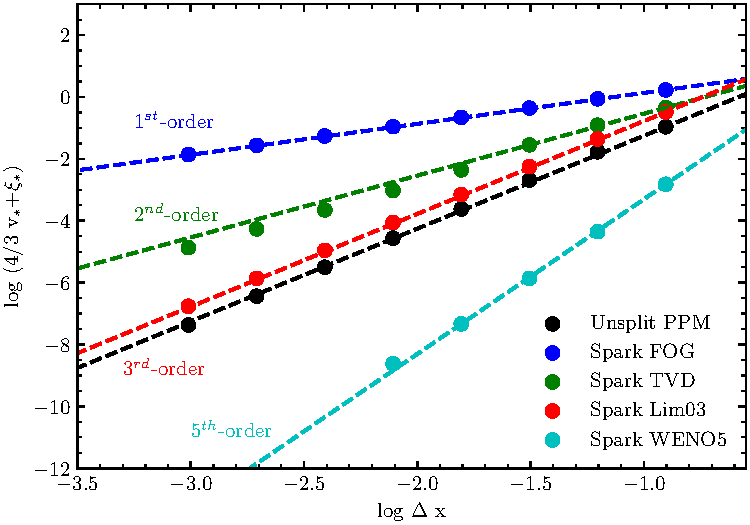
\includegraphics[width=3.25in]{figs/convergence}\\
    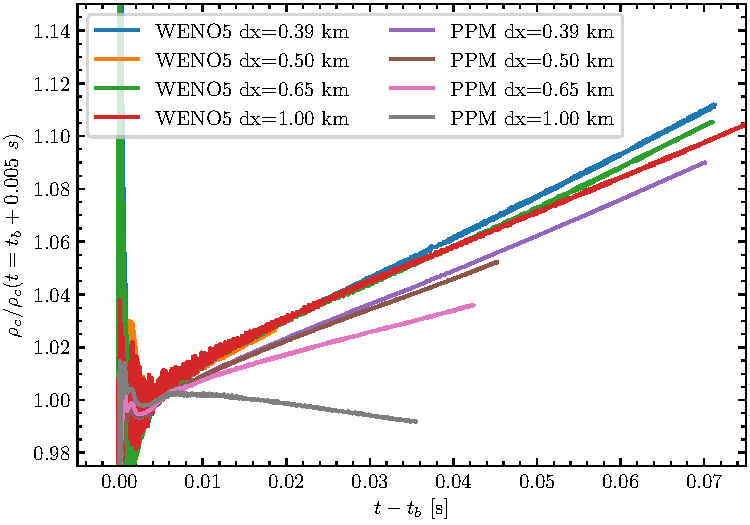
\includegraphics[width=3.25in]{figs/centralDens}
  \end{tabular}
  \caption{{\bf Top:} Rate of convergence of the numerical viscosity with grid resolution in a multidimensional sound wave advection test for \spark with various spatial reconstruction schemes along with that of \flash's unsplit PPM solver. For these tests, the time step CFL factor was set to 0.01 so that the truncation error second-order time integration scheme used in all cases was small. {\bf Bottom:} Post-bounce evolution of the normalized central density from 1D CCSN simulations at various resolutions for \spark with WENO5 and \flash's unsplit PPM solver.  The higher-order accuracy of WENO5 allows the neutron star to be held gravitationally at lower resolution than for PPM.}
  \label{fig:converge}
\end{figure}

%===========
\vspace{0.1in} \noindent {\bf Year 1 -- Total Request: 150M \mira core-hours; 9M \thet core-hours}
%===========

%%%%%%%%%
\subsection{High-fidelity 3D Simulations of Magnetorotational CCSNe}
\label{sec:Y1mrccsn}

In Year 1, we will carry out a set of high-resolution 3D CCSN simulations using \sparkmone using progenitors that include realistic rotation rates and magnetic field strengths.
We will construct our own 1D progenitor models using the open-source MESA code \citep{Paxton:2011, Paxton:2013, Paxton:2015} including rotational mixing instabilities and the Tayler-Spruit dynamo mechanism for magnetic field generation and angular momentum transport \citep{Spruit:2002, Heger:2005}.
Recent asteroseismology results for low-mass stars seem to indicate that the Tayler-Spruit mechanism may {\it underestimate} the amount of angular momentum transport out of rotating stellar cores \citep{Cantiello:2014}.
Thus, we will explore different coupling parameters in the stellar evolution models to construct cores of differing rotation rates for the same zero-age main sequence (ZAMS) masses.
Using MESA, we will simulate a range of ZAMS masses and angular momentum transport parameters.
From these models, we will select four to simulate in 3D using \sparkmone: ``low'' and ``high'' core rotation rates for a $\sim$10-\msun star and a $\sim$20-\msun star.
The exact initial models used will be decided based on the results of a set of 2D simulations using \sparkmone that will be completed prior to the start of Year 1.
The initial magnetic field strengths for the 3D simulations will be taken directly from the values achieved in the 1D MESA models.
The initial field geometry and spatial dependence will be a mix of poloidal and toroidal components guided by the 1D MESA models.

We will simulate in 3D these four models from the onset of core collapse through core bounce to $\sim$500 ms post-bounce.
Using AMR on a 3D Cartesian mesh, the maximum allowed refinement level will drop approximately logarithmically with radius from the center of the PNS.
The highest level of refinement will achieve a resolution of 650 m and cover the inner $\sim$80 km in radius, sufficient to keep the entire PNS and neutrinospheres at the same resolution.
The second level of refinement at resolution of 1.3 km will reach out to 160 km in radius, sufficient to encompass the entire post-shock gain region until the onset of explosive shock expansion in most cases.
This roughly equates to ``angular'' resolution varying between 0.47$^\circ$ and  0.93$^\circ$.
This is slightly coarser than the resolution we are using in the ``high''-resolution 3D simulations of our current INCITE project but our results from those simulations do not show dramatic differences at this reduced resolution (see Section \ref{sec:achievements}).
Furthermore, our use of higher-order WENO5 for the MHD solver will mitigate this substantially and, likely, result in a {\it reduced} numerical viscosity as compared to slight higher resolution simulations using PPM (see Fig. \ref{fig:converge}).
And this resolution is still substantially greater than the $\sim$2$^\circ$ angular resolution used by other comparable high-fidelity 3D simulations of CCSNe \citep[e.g.,][]{Melson:2015, Lentz:2015, Janka:2016}.
Each of the four 3D simulations will require 16M core-hours on \mira and 10 TB of online storage (see Section \ref{sec:performance}).
Including 2M \mira core-hours for development and testing, the total request for this milestone is 66M \mira core-hours and 40 TB of online storage.

In addition to the simulations on \mira, in Year 1 we will execute two 3D CCSN simulations using \sparkmone on \thet.
Using a Director's Discretionary allocation, we have already begun porting \sparkmone to \thet (see Section \ref{sec:readiness}).
Without any machine-specific tuning, our \sparkmone application shows a performance increase of {\it 4-5x per thread} on \thet as compared to \mira.
For these two simulations we will use the 10- and 20-\msun progenitors as above but without rotation or magnetic fields.
These will serve as interesting and relevant control cases for this Y1 milestone while also being an excellent opportunity to adapt and tune \sparkmone for \thet
For these two simulations we request a total of 8M \thet core-hours (26M \mira-equivalent core-hours) and 20 TB of online storage.
Plus an additional 1M \thet core-hours for development and testing, the total request for \thet in Y1 is 9M core-hours (29.25M \mira-equivalent core-hours).


\todo{What's the payoff?}

%%%%%%%%
\subsection{3D Simulations of Iron Core Collapse in Rotating Stars}
\label{sec:Y1progen}

One of the most remarkable and exciting results of recent 3D simulations of the CCSN mechanism is the discovery that  realistic non-spherical structure in the progenitor star can have a dramatic impact \citep{Couch:2013b, Couch:2015, Couch:2015a, Muller:2015, Muller:2017}.
The breaking of spherical symmetry is manifest in the turbulent convection driven by nuclear burning in the cores of massive stars.
As a massive star nears collapse, strongly convective burning in the Si and O shells surrounding the iron core can reach speeds of nearly 1000 km s$^{-1}$ and is characteristically very large in spatial scale \citep{Arnett:2011, Couch:2015a, Muller:2016a}.
These convective perturbations will reach the stalled shock shortly after core bounce and can aid neutrino-driven explosions by either enhancing the strength of post-shock turbulence \citep{Couch:2015} or causing large scale ``forced shock deformations'' \citep{Muller:2017}, or both.
These results serve to remind us that CCSN mechanism simulations are initial value problems and that the details of our initial conditions matter tremendously!
Our work inaugurated the era of detailed investigation into the impact of 3D progenitor structure on the CCSN mechanism \citep{Couch:2013b, Couch:2015a}.
As part of this INCITE project we will substantially expand the investigation into realistic progenitor structure for use in CCSN simulations.

We propose to carry out a series of new, high-fidelity 3D simulations of the final minutes of stellar evolution to the point of iron core collapse.
As part of the pending SciDAC TEAMS collaboration, we are working with M. Zingale to adapt the Maestro low-mach number code \citep{Almgren:2007} to massive stellar cores.
This will allow simulation of much longer time scales than currently possible \citep[a few minutes;][]{Couch:2015a, Muller:2016a}.
In the meantime, as part of this INCITE project we will continue the use of \flash in simulating the minutes up to core collapse in 3D.
For these simulations we will use the \spark MHD solver \citep{Couch:2017} and include rotation and magnetic fields {\it for the first time ever} in a 3D CCSN progenitor simulation.
Specifically, we will use the four 1D MESA progenitor models selected for 3D CCSN simulation in Section \ref{sec:Y1mrccsn}, initialized in 3D approximately five minutes prior to core collapse.
We will follow the final build up of the iron core to its critical mass and ensuing collapse using an approximate 21-isotope nuclear network \citep{Couch:2015a}.
We have recently made improvements to this network's handling of weak interactions that bring the evolution into better agreement with the 1D evolution from the MESA code.
We are currently simulating non-rotating, non-magnetic progenitors with this application in 2D and 3D.

Using AMR in Cartesian coordinates, we will use and approximate angular resolution of $\sim$0.5$^\circ$, as in \citep{Couch:2015a} and finer than that used by \citep{Muller:2017}.
Additionally, we will use \spark's high-order WENO5 reconstruction to achieve much lower numerical viscosity than PPM at comparable resolution.
Each such simulation will require 5M core-hours on \mira, for a total of 20M core-hours for the four simulations.
We request 10 TB of online storage for these simulations.
We will make the final 3D progenitor models publicly available and provide reader and interpolation routines in Fortran and Python for accessing the data so that other groups can readily incorporate these new 3D progenitors into their CCSN simulations.
We will incorporate these first-of-their-kind 3D magnetorotational progenitor models into our CCSN mechanism simulations in Year 2 and 3 of this INCITE project.

%%%%%%%%
\subsection{High-resolution Simulation of Magnetorotational Turbulence in CCSNe}
\label{sec:Y1hero}

The neutrino-heated gain region in CCSNe is highly turbulent with physical Reynolds numbers $\sim$10$^{17}$.
Numerous recent works have pointed out that the larger numerical viscosities due to finite resolution in current 3D CCSN simulations is such that the effective {\it numerical} Reynolds numbers may only be a few hundred \citep{Couch:2015, Abdikamalov:2015, Radice:2015, Radice:2016}, arguably not even turbulent.
This could have a significant impact on the dynamics of the simulations, including a ``bottleneck'' effect preventing an efficient cascade of turbulent kinetic energy from large to small scales \citep{Hanke:2012, Couch:2013a, Abdikamalov:2015, Radice:2016}.
Since the transition from stalled shock to explosion in 3D is attended by the appearance of the large-scale buoyant plumes behind the shock \citep{Dolence:2013, Muller:2017}, this bottleneck could have a crucial impact on the qualitative outcome of CCSN simulations.

The highest-resolution 3D CCSN simulations with high-fidelity neutrino transport have only used $\sim$1 km resolution in the gain region \citep{Roberts:2016, OConnor:2017}.
The parameterized simulations \citet{Radice:2016} show that this resoulution is not sufficient to correctly capture the turbulent cascade, though it it close to correctly calculating the turbulent kinetic energy on large scales.
We propose to carry out the highest resolution neutrino-radiation hydrodynamic CCSN simulation yet.
This simulation will have critical value as a validation of the resolution used in current 3D CCSN simulations.
For this simulation, we will allow the entire post-shock region to be refined up to a resolution of 650 m, twice the resolution of our fiducial model set (Section \ref{sec:Y1mrccsn}).
Coupled with the higher-order WENO5 scheme we will use, this simulation should achieve the highest numerical Reynolds number of any 3D CCN simulation yet.
We will careful study the character and properties of the gain region turbulence in this simulation and compare to our fiducial models.
We will select the initial based on the results of the simulations in Section \ref{sec:Y1mrccsn}.
This simulation will comprise approximately 100 million computational zones.
We will simulate approximately 500 ms of post-bounce evolution, bringing the request for this simulation to 60M core-hours and 40 TB of online storage.

% \subsection{Realistic CCSN Nucleosynthesis}
% \label{sec:nucleo}
%
% CCSNe are principally responsible for the production of elements heavier than Lithium throughout the universe.
% The nucleosynthetic yields from CCSN simulations is a key quantity that can be directly compared to observations and laboratory measurements of cosmic abundances.
% As such, we propose to compute detailed nucleosynthesis from our CCSN simulation results.
% This will be accomplished as a post-processing step using large ($\sim$1000 isotopes) nuclear reaction networks furnished by Co-I's Arcones and Fr\"ohlich.
% The input for the nuclear reaction networks will be passive tracer particle data that records thermodynamic trajectory information from our FLASH CCSN simulations.
% FLASH already includes a well-developed, efficient passive particles framework that has been used extensively in the calculation of nucleosynthesis in Type Ia supernova simulations \citep[e.g.,][]{Long:2014dv}.
%
% The nucleosynthesis during the first second post-bounce is interesting and scientifically valuable by itself, but we will also go beyond this short time.
% In collaboration with Co-I Arcones and her graduate student, we have adapted our FLASH CCSN application to smoothly transition from the high-density NSE EOS to a reduced nuclear reaction network and appropriate EOS at low densities.
% %FLASH includes several nuclear reaction networks to choose from, but in order to make the transition from the four-species NSE at high densities, we have added the ability to incorporate an additional neutron-rich tracer nucleus to the networks that allows us to match the $\bar A$ and $\bar Z$ of the NSE network making for a smooth EOS transition.
% %At high densities, the multispecies approximate network is maintained in NSE through use of an appropriate NSE solver.
% The ability to accurately simulate the nucleosynthesis and thermodynamics of low-density regions allows us to extend our CCSN simulations to late times and large radii, even to follow the development of explosions through the entire progenitor \citep[e.g.,][]{{Kifonidis:2003hs}, Couch:2009bu, {Couch:2011cf}}.
% With these multidimensional simulations we will be able to take a remarkably detailed look at nucleosynthesis and mixing in the earliest stages of the formation of a young CCSN remnant \citep{Hammer:2010di}.
% Comparison to observations of galactic CCSN remnants, such as Cas A \citep{Grefenstette:2014ds}, will be made as well as comparison to cosmic chemical abundances.
%
% The post-processing nuclear reaction networks are embarrassingly parallel, requiring no interprocess communication.
% The large number of particles that will be required for each 3D simulation ($\sim$millions) will easily make these Capability class simulations, though only short runtimes will be needed.
% For this we request 5M MSU.
% The 3D simulations of long timescale CCSN mixing, using the methods developed in \citet{Couch:2011cf}, will require a roughly equal amount of computing resources for each decade in radius simulated.
% These simulations will not require neutrino transport and so are relatively inexpensive.
% Restricting ourselves to compact progenitor stars ($R_* \sim 10^{6}$ km), we plan two 3D whole-star simulations each, requiring about 5M MSU.  The total request for the nucleosynthesis and 3D whole-star simulations is then 15M MSU.

\vspace{0.1in} \noindent {\bf Year 2 -- Total Request: 150M {\it Mira} core-hours; 18M \thet core-hours}


\subsection{3D Multi-Dimensional Neutrino Transport Sims with Enhanced Physics}
\label{sec:enhancedM1}

In the third year of the project we will extend our M1 calculations to include velocity terms and inelastic scattering in the transport equations.
This will dramatically increase the expense of the simulations, but as \citet{Lentz:2012fy} point out, these terms can have an important impact on the results of CCSN simulations.
These calculations will push forward the leading edge of sophistication in CCSN simulation.
The realistic neutrino transport, coupled with our handling of the MRI, will make these the most physically-complete and accurate CCSN simulations yet attempted.
The coupled-energy group version of the M1 code is already developed in GR1D.
Early tests indicate that the expense is approximately four times the current M1 scheme.
%Given the great cost, we will conduct this simulation in reduced resolution.
We will simulate a rotating, magnetic progenitor and include the MRI sub-grid model.
For $dx_{\rm min} = 0.5$ km and effective angular resolution of $0.55^\circ$ the simulation will consist of 53 million zones and 600,000 time steps to simulation 500 ms of post-bounce evolution, costing 70M MSU.
We request a further 5M MSU for testing and development of the energy-coupled M1 code.

% \subsection{Monte Carlo Radiative Transfer of 3D CCSN Simulations}
% \label{sec:radtrans}
%
% \todo{Talk about Sedona and Kasen?}
%
% In Y3 of this project, we will make direct comparison to EM observations of CCSNe through the calculation of light curves and spectra from our simulations.
% We will utilize the newly-developed Implicit Monte Carlo/Discrete Diffusion Monte Carlo radiative transfer code, SuperNu \citep{Wollaeger:2013ix}.
% SuperNu is presently being extended to 3D by utilizing the very same AMR grid package as FLASH, making compatibility between the two codes straight-forward.
% We will use as input for these calculations the hydrodynamic and nucleosynthetic results of the previous two years.
% Being a Monte Carlo method, SuperNu is inherently embarrassingly parallel, though testing in 1D indicates a very large number of Monte Carlo particle packets are necessary for good signal-to-noise.
% Thus we anticipate these calculations to be expensive for 3D data and request an allocation of 25M MSU for our Y3 3D radiative transfer calculations.


% \begin{wrapfigure}[17]{r}{3.5in}
% \includegraphics[width=3.7in, trim= 0in 0in 0in .27in, clip]{data/m25}
% \caption{MRI characteristic parameters from a 1.5D collapse simulation of a 25 $M_{\odot}$ star at 70 ms post-bounce.
% Within the PNS ($\lesssim 40$ km) entropy and composition gradients stabilize the MRI.}
% \label{fig:mri}
% \end{wrapfigure}
